\documentclass{article}
\usepackage{graphicx}
\usepackage{subcaption}
\usepackage{float}

\begin{document}

\title{LU Factorization Analysis}
\author{Your Name}
\date{\today}
\maketitle

\section{Factorization Accuracy vs. Problem Size}
\begin{figure}[H]
    \centering
    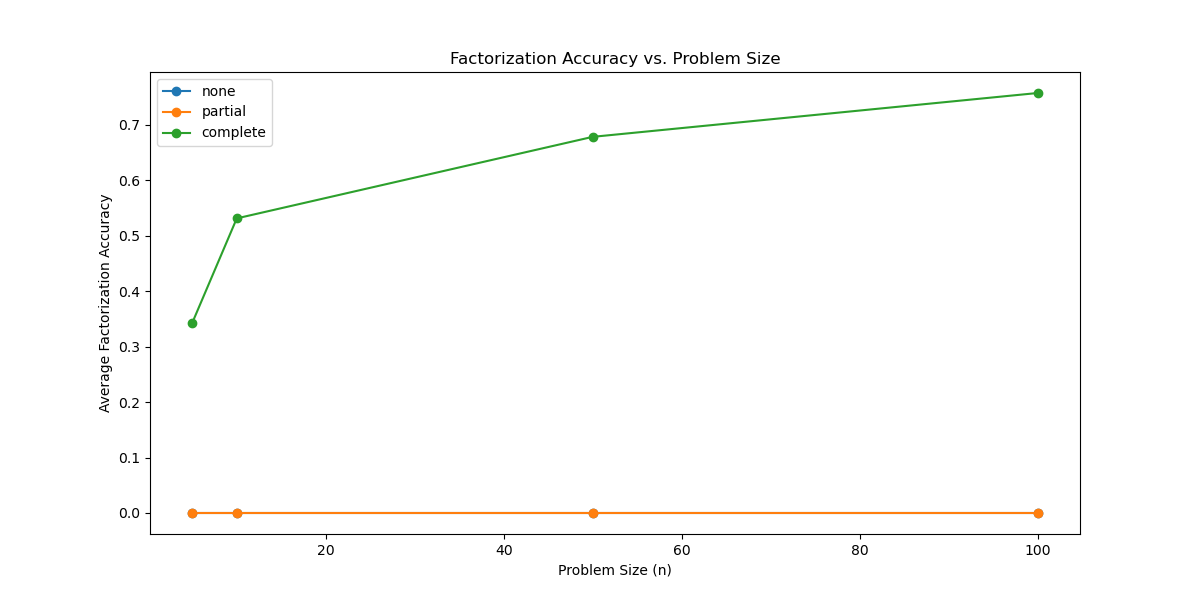
\includegraphics[width=0.7\textwidth]{acc_over_n.png}
    \caption{Factorization Accuracy vs. Problem Size}
\end{figure}

\section{Growth Factor vs. Problem Size}
\begin{figure}[H]
    \centering
    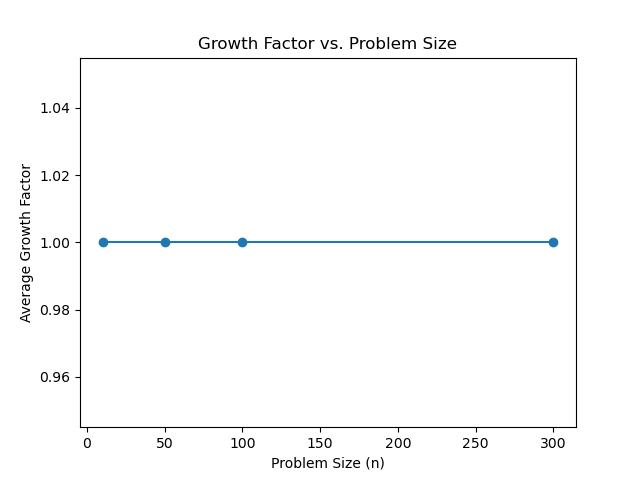
\includegraphics[width=0.7\textwidth]{grow_fac.png}
    \caption{Growth Factor vs. Problem Size}
\end{figure}

\section{Execution Time vs. Problem Size}
\begin{figure}[H]
    \centering
    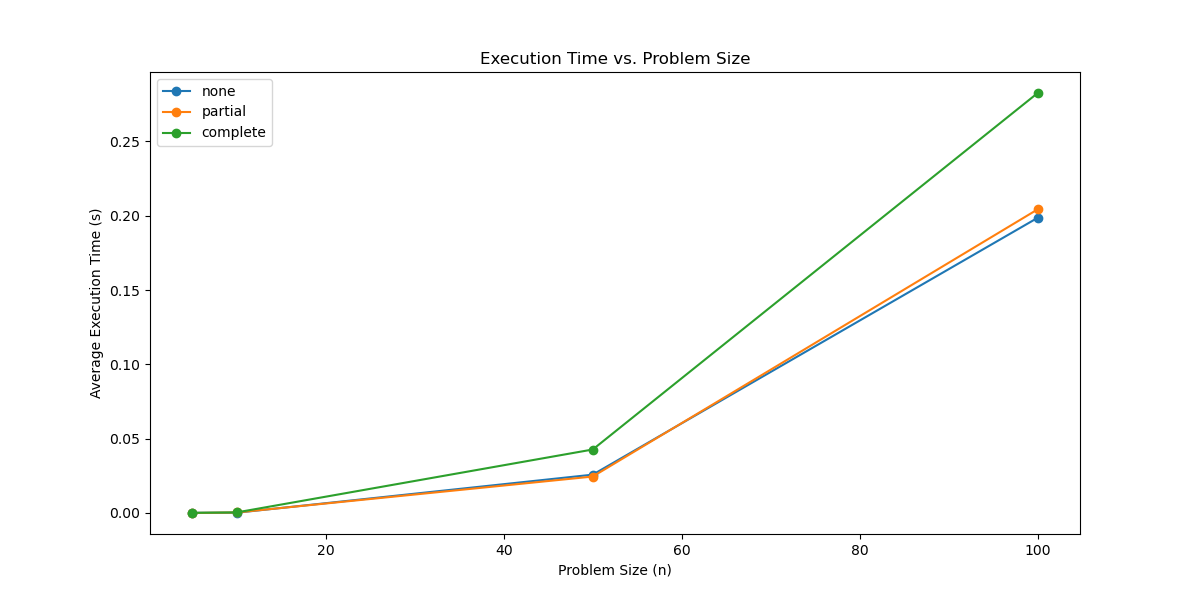
\includegraphics[width=0.7\textwidth]{ex_time.png}
    \caption{Execution Time vs. Problem Size}
\end{figure}

\end{document}
